	\documentclass{article}
	\usepackage{graphicx}
	\usepackage{curves}	
	\usepackage{amsmath}	
	
	\begin{document}
	
\title{A Brief Introduction to Log Polar Mapping}
\author{Fabio Berton}
\maketitle
\section{Notation}
\label{sec:Notation}

Given a log polar pixel $(\rho,\theta)$, the general formulas to compute its cartesian position are:
	
\begin{equation}
	\begin{cases}
	R = \lambda^{\rho} \cdot r_{0} \\
	\omega = \frac{2\pi\theta }{\Theta} \\
	\end{cases}
\end{equation}

where:

$R$ is the distance between the center of the receptive field (RF) and the center of the mapping.

$\omega$ is the counter-clockwise angular distance of the center of the RF from the horizontal axis.

$\lambda$ is the ratio between the widths of two subsequent rings.

$r_{0}$ is the radius of the ring with index $\rho = 0$.

$\Theta$ is the number of RF's per ring.

%\begin{tabbing}
%XXX\=\kill
%$R$ \> distance \ between the center of the receptive field (RF) and the center of the mapping.\\
%$\omega$ \> angular distance of the RF from the horizontal axis.\\
%\end{tabbing} 
\paragraph{}

 Note that the log polar domain is intended as a discrete domain, so $(\rho,\theta)$ represents the pixel covering the rectangular area delimited by $(\rho,\theta)$ and $(\rho+1,\theta+1)$. So the cartesian coordinates of the point will be:

\begin{equation}
	\begin{cases}
	x=R \cdot \cos (\omega)\\
	y=R \cdot \sin (\omega)\\
	\end{cases}
\end{equation}

which is:
\begin{equation}
	\begin{cases}
	x=\lambda^{\rho} \cdot r_{0} \cdot \cos (\frac{2\pi\theta }{\Theta})\\
	y=\lambda^{\rho} \cdot r_{0} \cdot \sin (\frac{2\pi\theta }{\Theta})\\
	\end{cases}
\end{equation}

The inverse transformation is given by
\begin{equation}
	\begin{cases}
	\rho=\log_{\lambda}\frac{R}{r_{0}}= \log_{\lambda}\frac{\sqrt{x^2+y^2}}{r_{0}}\\
	\theta=\frac{\Theta\omega}{2\pi}=\frac{\Theta}{2\pi}\arctan\frac{y}{x}\\
	\end{cases}
\end{equation}

\begin{figure}[htb]
	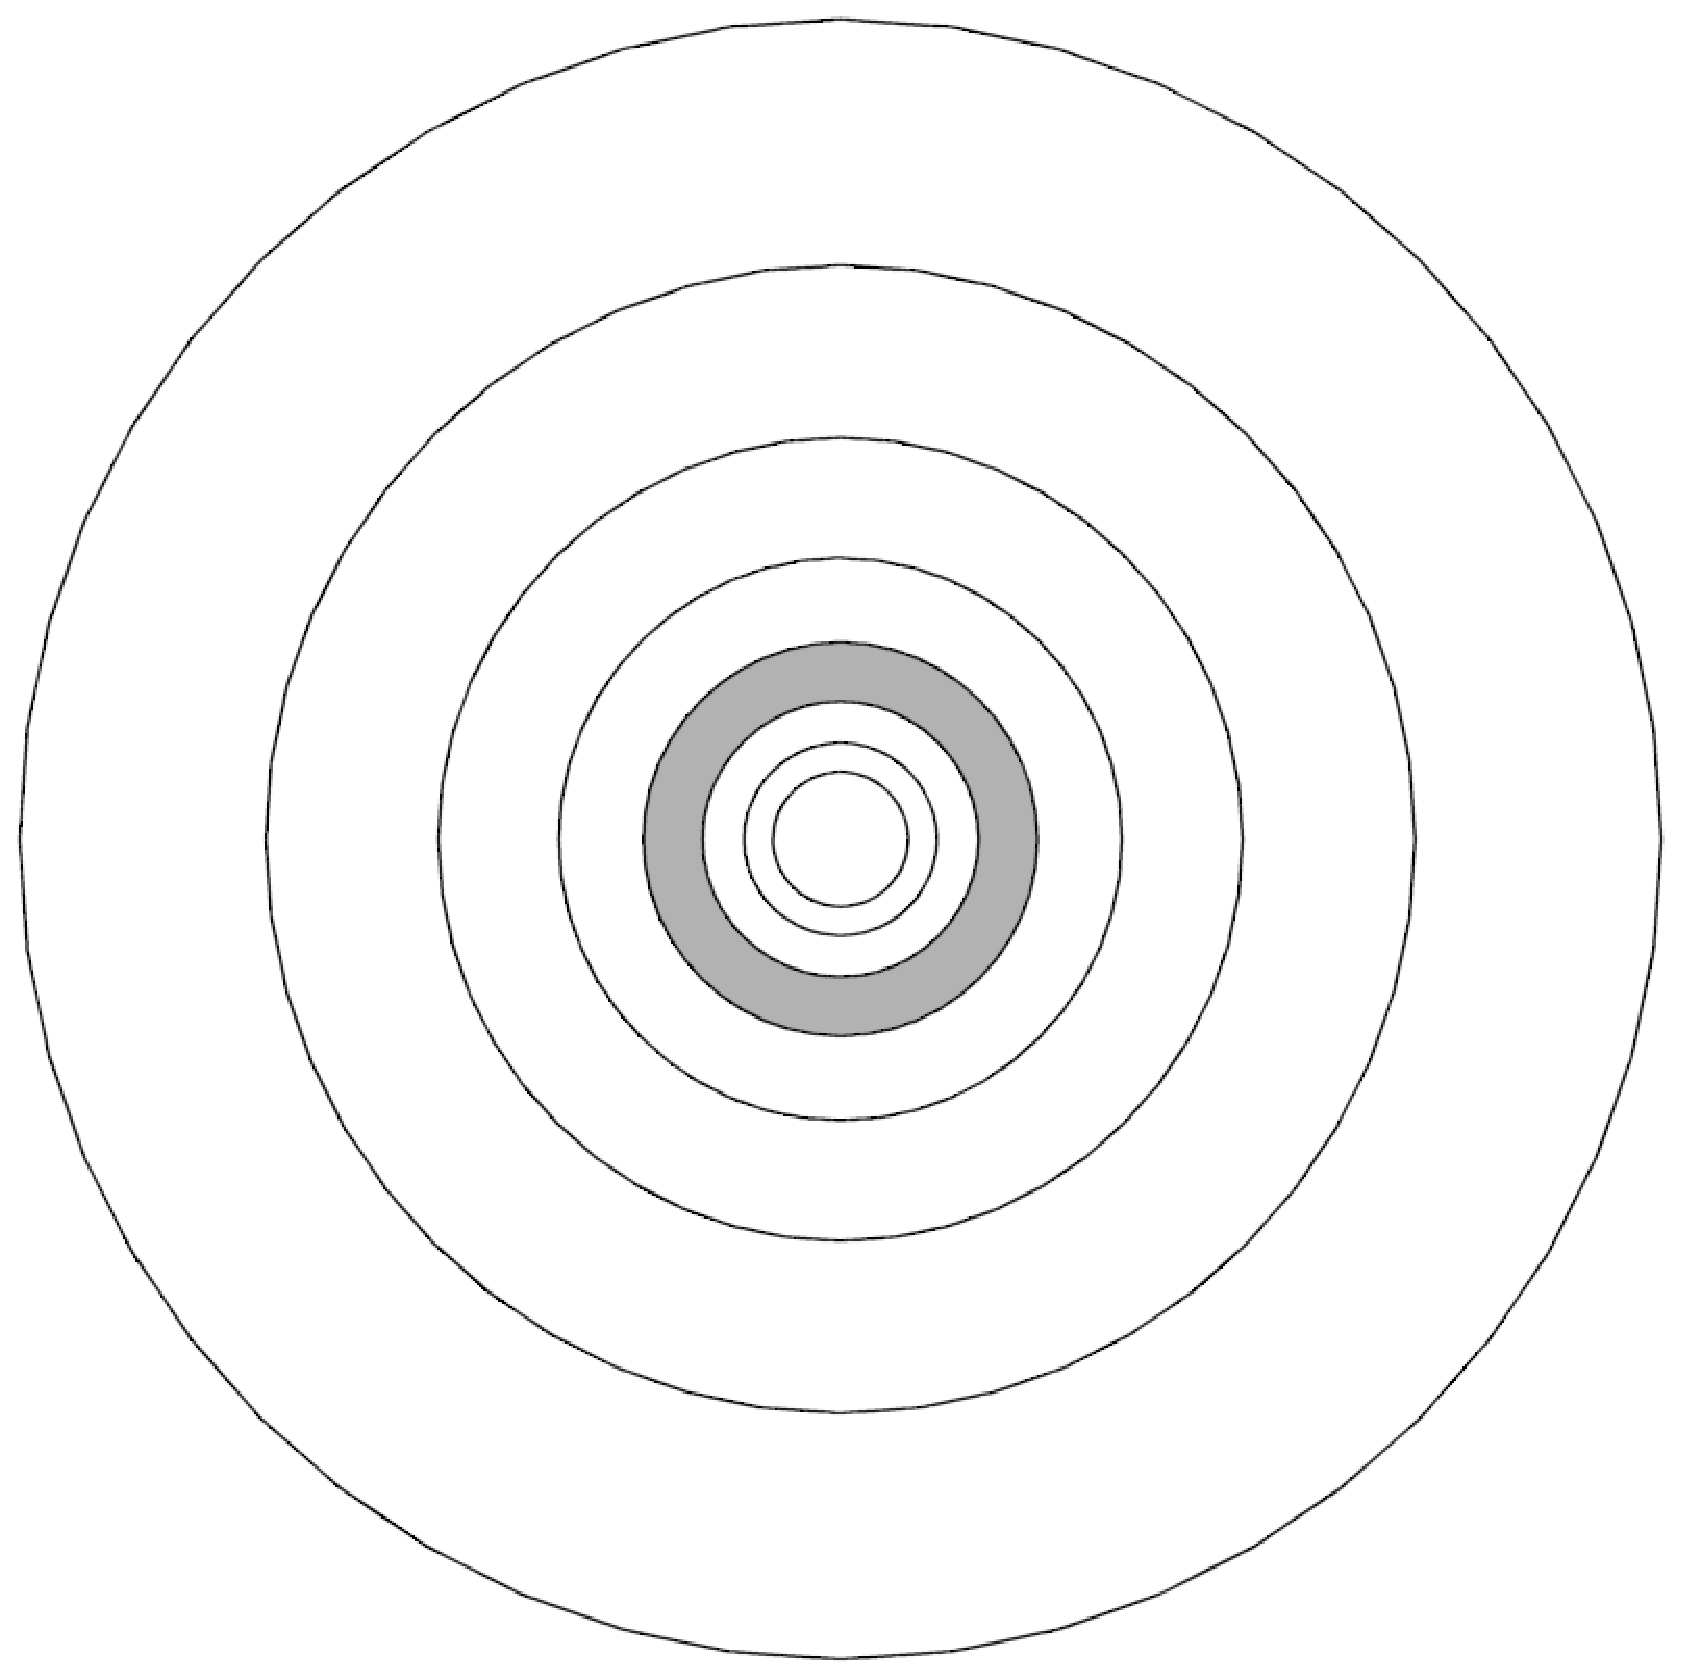
\includegraphics[width=0.30\textwidth]{PureLog.eps}
	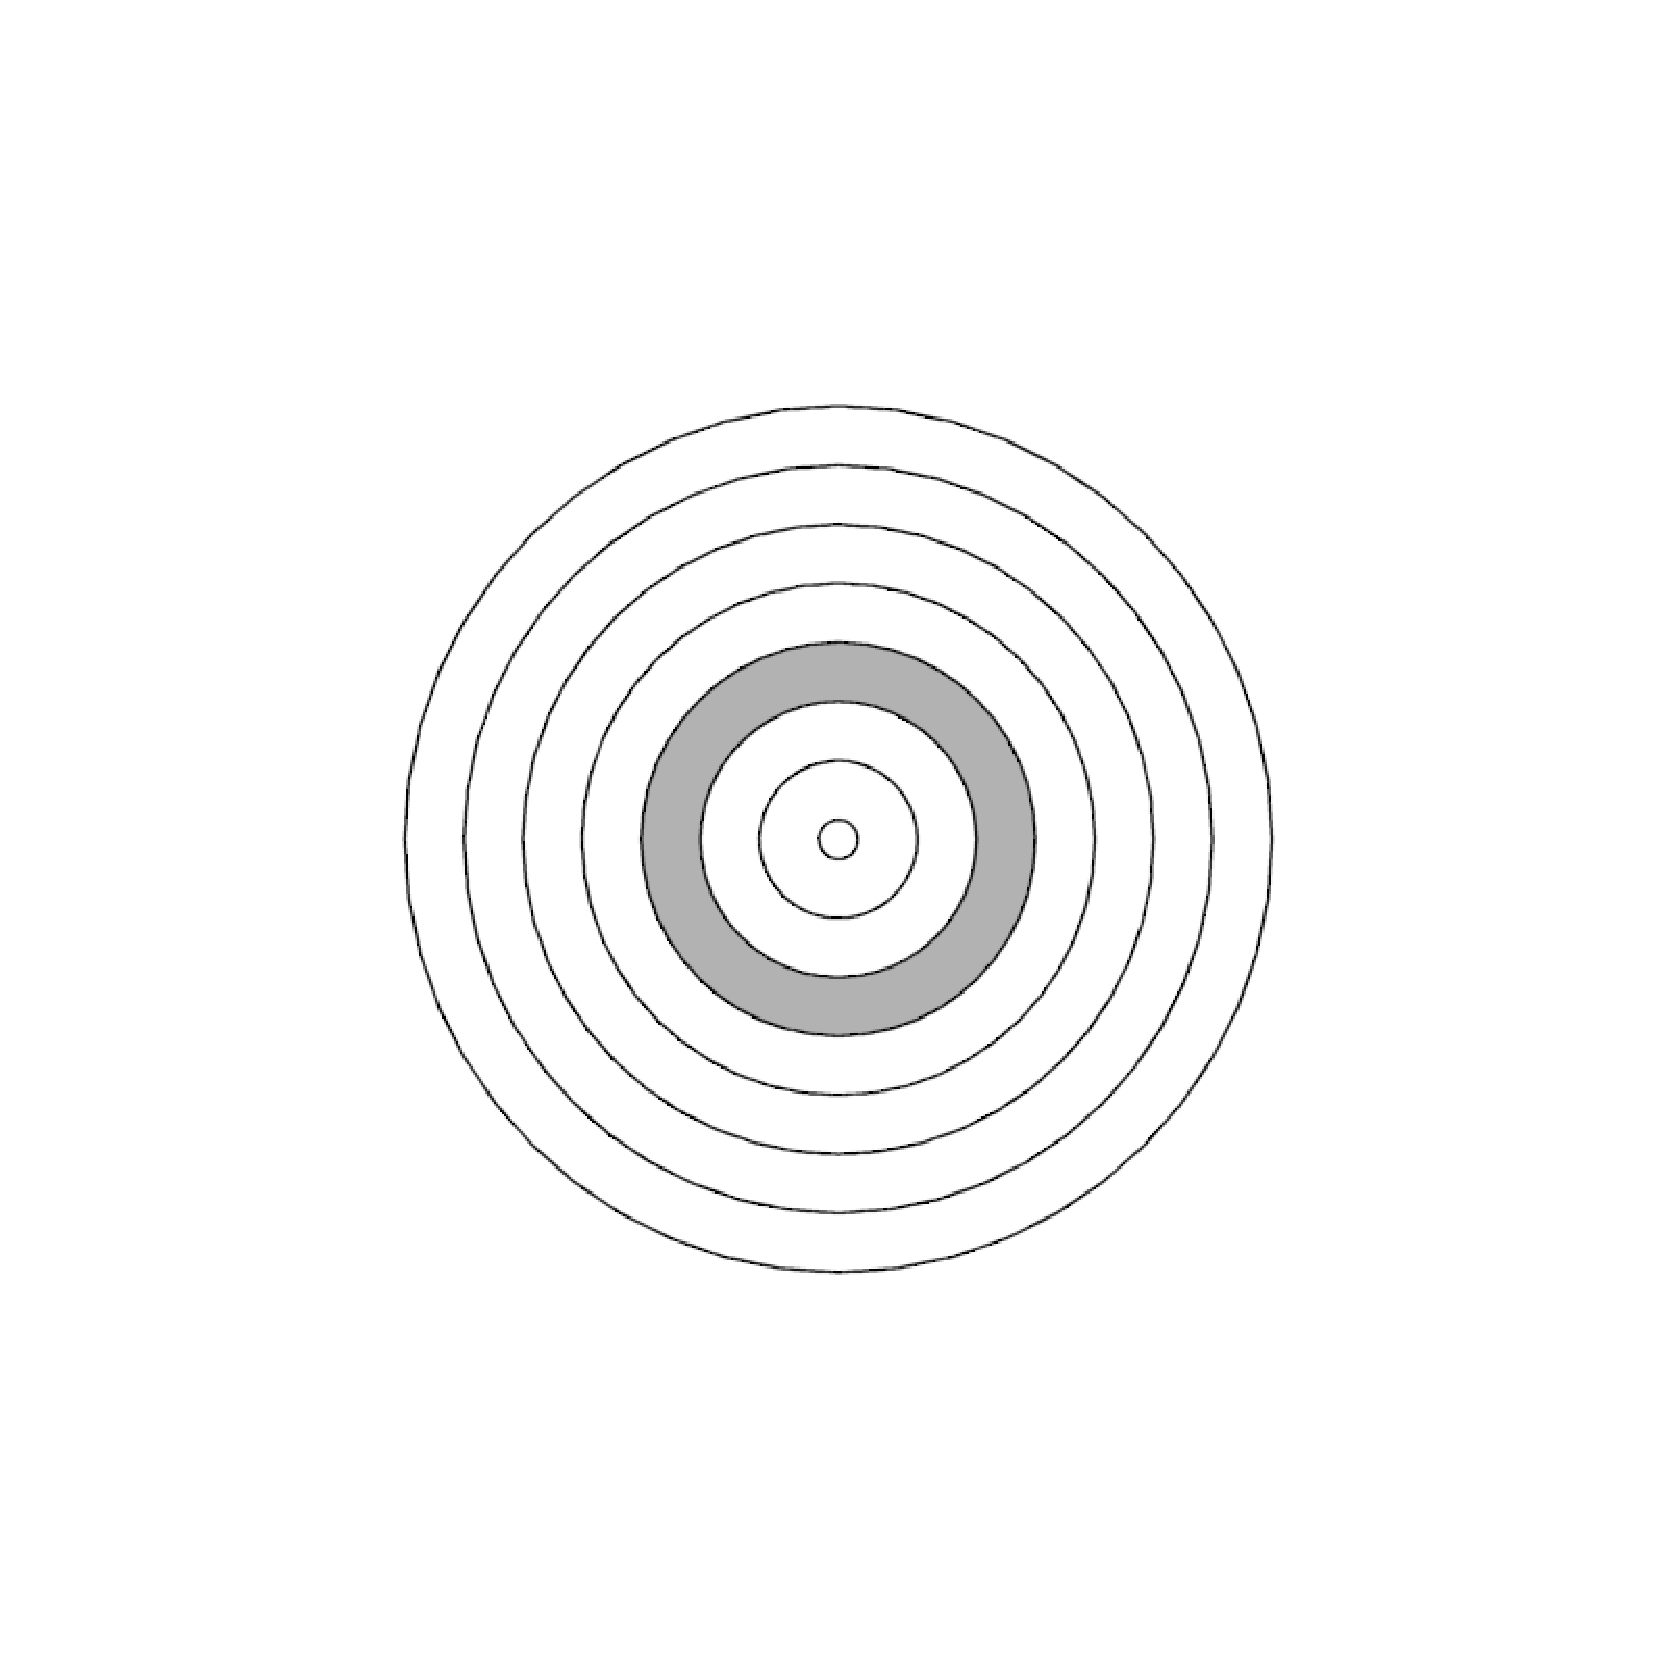
\includegraphics[width=0.30\textwidth]{LinPolar.eps}
	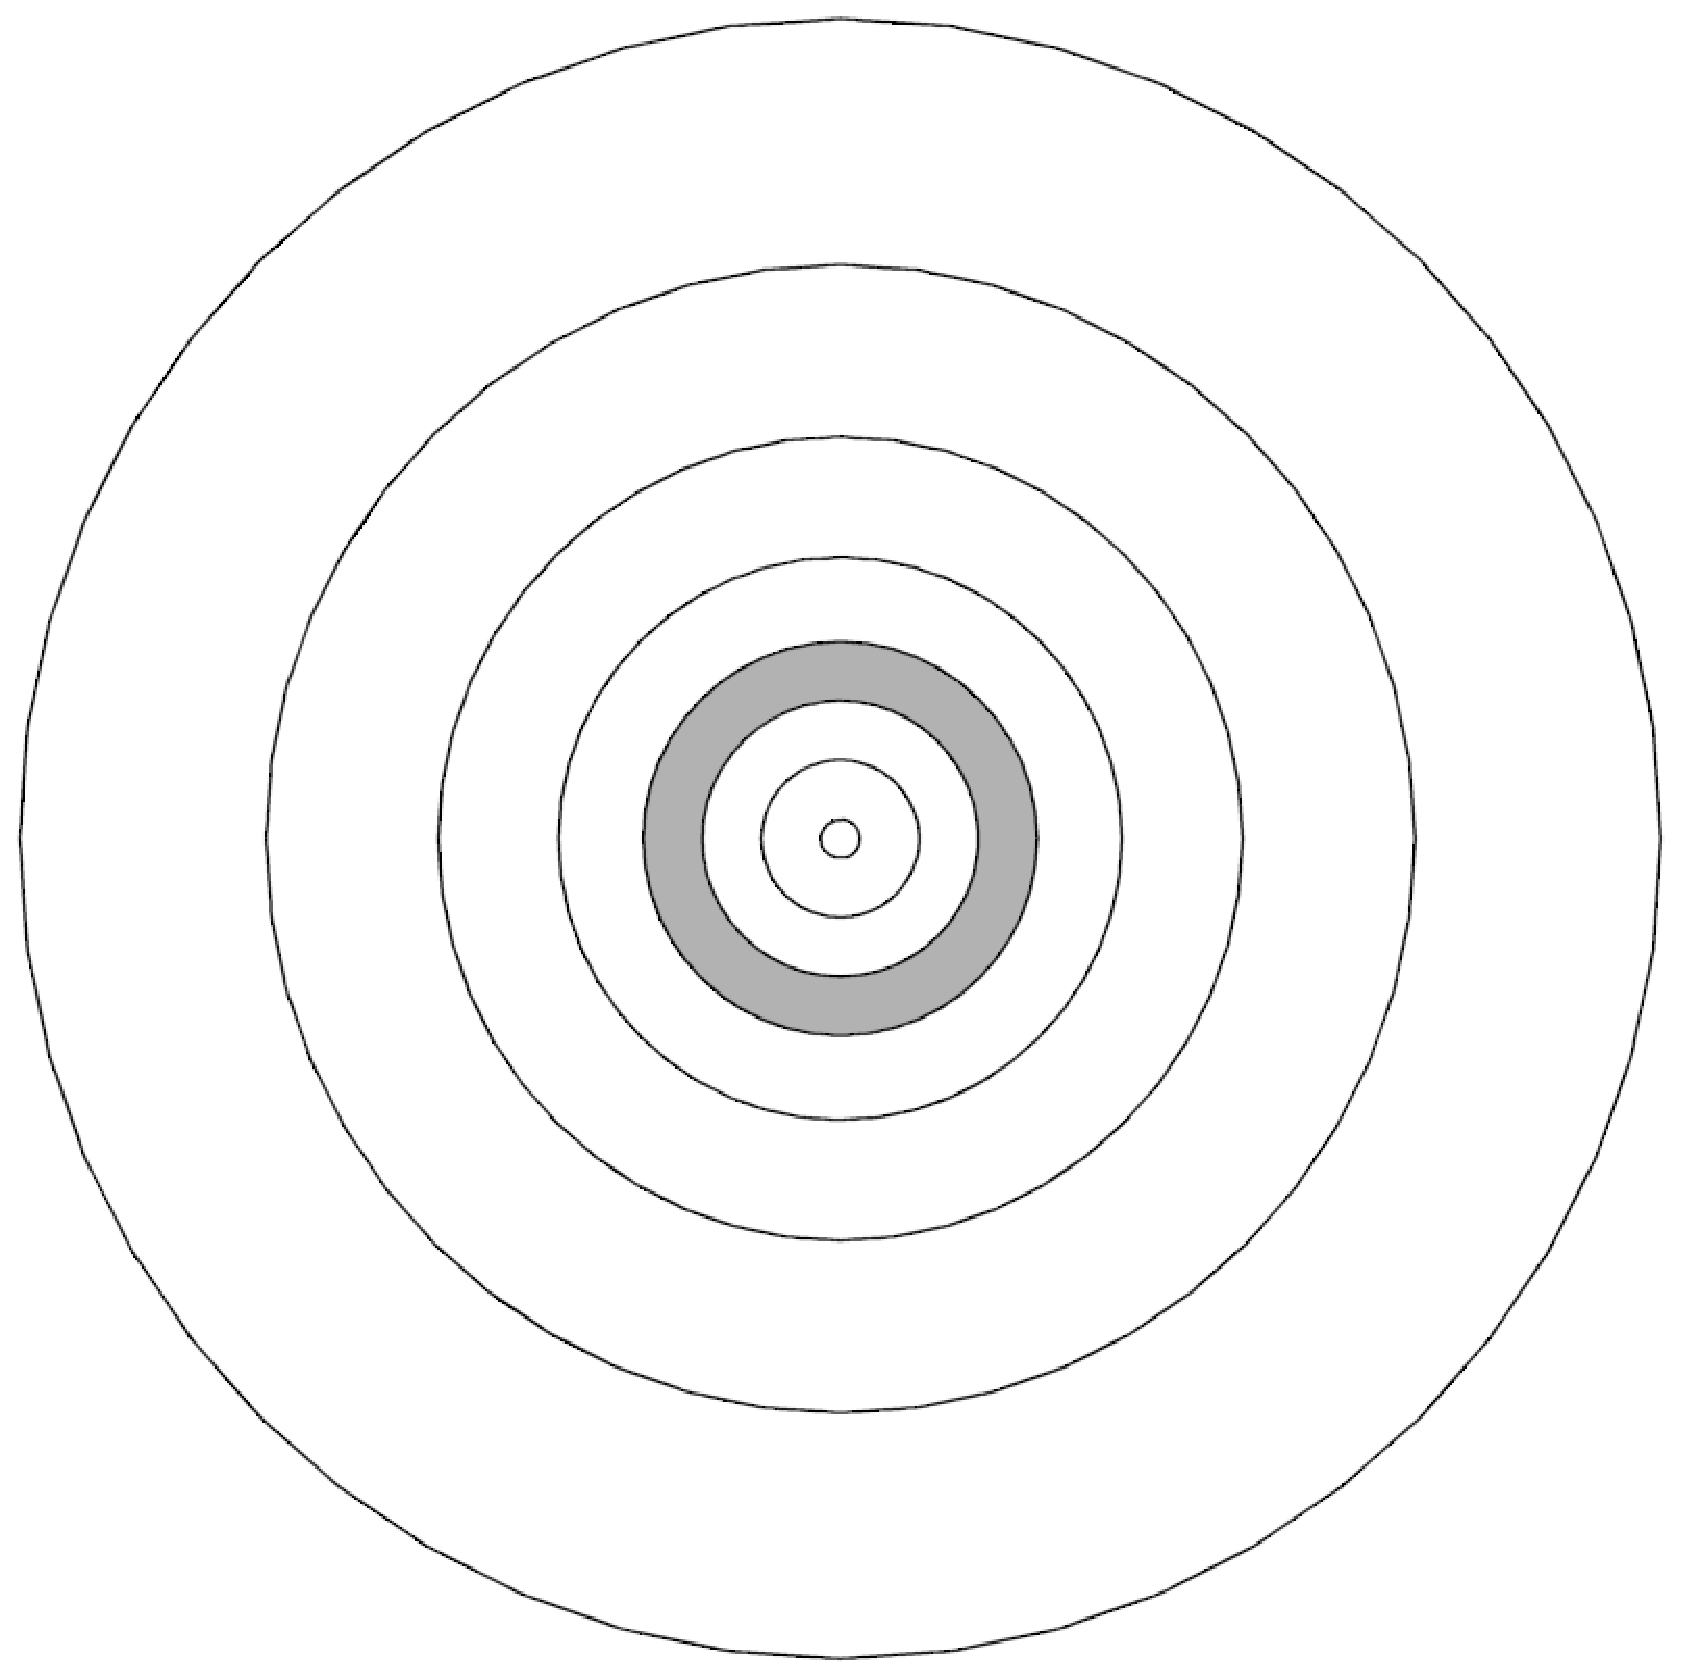
\includegraphics[width=0.30\textwidth]{LogPolarAndFovea.eps}
	\caption{The Mapping outside the gray ring is pure logarithmic (left), while inside of it is pure linear polar (center). The overlapping of the two mappings gives the right image.}
	\label{fig:LinandLogPolar}
\end{figure}


From the previous formulae is easy to notice that there is a discontinuity in the origin: since the width of the rings when approaching the origin tends to zero, it is impossible to cover the central area with a finite number of receptive fields. 
Then, a common strategy is to cover the fovea with a linear polar distribution of RF's, defined by the following:

\begin{equation}
	\begin{cases}
	R = \rho +\varepsilon\\
	\omega = \frac{2\pi\theta }{\Theta} \\
	\end{cases}
\end{equation}

The term $\varepsilon$ is added in order to have a perfect overlap between the last ring in fovea for the two mappings (linear and logarithmic, see figure).


%\begin{eqnarray}
%	\begin{matrix} 0 & 1 \\ 1 & 0 \end{matrix}
%	R(\rho) = \lambda^{\rho}\cdot r_{0}\\
%\end{eqnarray}
	
\section{Computing the Logarithm Index}
\label{sec:ComputingTheLogarithmIndex}

	We want to compute the logarithm index $\lambda$, given the number of pixels per ring $\Theta$. Let's set the following:
	
\begin{eqnarray}
	\overline{AB}=2r_{n}\\
	\overline{A'B'}=2r_{n-1}\\
	\overline{OA}=\overline{OB}=R_{n}\\
	\overline{OA'}=\overline{OB'}=R_{n-1}
\end{eqnarray}

\begin{figure}[htb]
%	\setlength{\unitlength}{1mm}
%	\linethickness{0.8pt}
%	\begin{picture}(0,0)(40,40)
%		\put(0,0){\bigcircle[0]{6.962}}
%		\put(0,0){\line(1,0){40.335}}
%		\put(0,0){\qbezier(-3.481,0)(-2.493,0.156)(95.288,15.643)}
%		\put(8.481,0){\bigcircle[0]{10}}
%		\put(18.481,0){\bigcircle[0]{10}}
%		\put(28.481,0){\bigcircle[0]{10}}
%		\put(40.335,0){\bigcircle[0]{13.709}}
%	\end{picture}
	\centering
		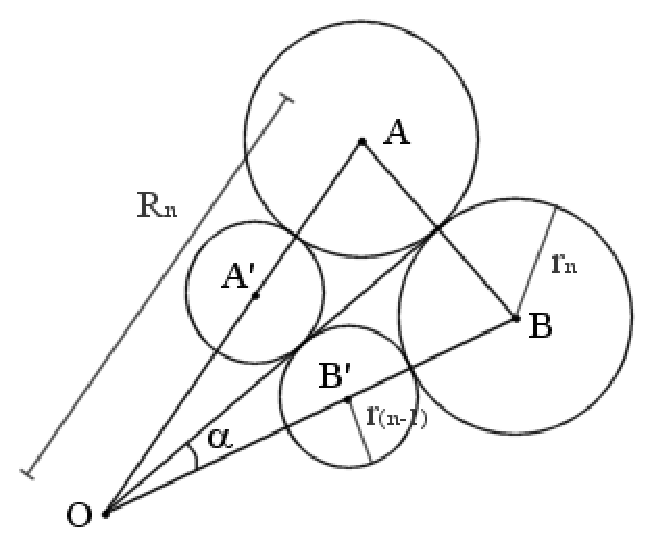
\includegraphics[width=0.50\textwidth]{Image1.eps}
	\caption{How to compute the Log Index}
	\label{fig:Image1}
\end{figure}


We can easily see that $r_{n-1}=R_{n-1}\sin(\alpha)$ and $2\alpha = \frac{2\pi}{\Theta}$. Considering that the sum $r_{n-1}+r_{n}$ equals the difference $R_{n}-R_{n-1}$ and $r_{n}=\lambda\cdot r_{n-1}$. So:


\begin{eqnarray}
	r_{n}+r_{n-1}=R_{n}-R_{n-1}\\
	\lambda\cdot r_{n-1}+r_{n-1}=\lambda\cdot R_{n-1}-R_{n-1}\\
	r_{n-1}\left(\lambda+1\right)=R_{n-1}\left(\lambda-1\right)\\
	r_{n-1}=R_{n-1}\cdot\frac{\lambda-1}{\lambda+1}\\
	R_{n-1}\sin(\alpha)=R_{n-1}\cdot\frac{\lambda-1}{\lambda+1}\\
	\sin\alpha=\frac{\lambda-1}{\lambda+1}\\
	\lambda(1-\sin\alpha)=1+\sin\alpha\\
	\lambda = \frac{1+\sin\alpha}{1-\sin\alpha}\\
	\lambda = \frac{1+\sin\frac{\pi}{\Theta}}{1-\sin\frac{\pi}{\Theta}}
\end{eqnarray}

%\begin{table}
%	\centering
%		\begin{tabular}[]{ccc}
%			$\Theta$	& $\lambda$ & $F$\\	
%			\\	
%			126	& 1.0511362454481 & 20\\		
%			128	& 1.0503173055397 & 20\\		
%			252	& 1.0252473708587 & 40\\		
%			256	& 1.0248479997517 & 41\\		
%			504	& 1.0125447517139 & 80\\		
%			512	& 1.0123475323324 & 81\\		
%		\end{tabular}
%	\caption{Some Values for $\lambda$ and $F$}
%	\label{tab:SomeValuesForLambda}
%\end{table}
\section{Computing the Fovea Size}
\label{sec:ComputingTheFoveaSize}
	
\begin{figure}[htbp]
	\centering
		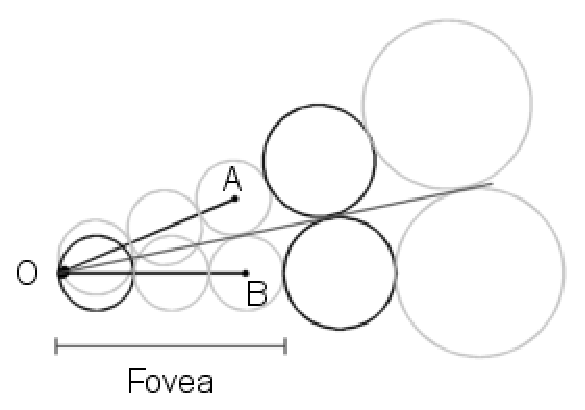
\includegraphics[width=0.50\textwidth]{Image2.eps}
	\caption{How to compute the Fovea Size}
	\label{fig:Image2}
\end{figure}

The Fovea is the constant resolution part of the mapping. So the size of each receptive field (when circular), here is constant. In the figure, $O$ is the center of the mapping, the first three receptive fields belong to fovea, and they all have radius $r_{f}$. The first receptive field out of the fovea will have a radius of $\lambda\cdot r_{f}$, the second $\lambda^{2}\cdot r_{f}$ and so on. Then the distance $\overline{OA}$ will be $(2F-1)\cdot r_{f}$, where $F$ is the number of receptive fields in the fovea, thus $(2F-1)\cdot r_{f}\cdot sin(\alpha)=r_{f}$. Since $sin(\alpha)=\frac{\lambda-1}{\lambda+1}$, we will have:
\begin{eqnarray}
	(2F-1)\cdot r_{f}\cdot \sin(\alpha)=r_{f}\\
	(2F-1)\cdot \sin(\alpha)=1\\
	(2F-1)\cdot \frac{\lambda-1}{\lambda+1}=1\\
	(2F-1)\cdot \lambda-1=\lambda+1\\
	2F\lambda-\lambda-2F+1=\lambda+1\\
	2F\lambda-2F=2\lambda\\
	F\lambda-F=\lambda\\
	F=\frac{\lambda}{\lambda-1}
\end{eqnarray}

In the same way:
\begin{eqnarray}
	\overline{OA'}=2F+\lambda\\
	(2F+\lambda)\cdot \sin(\alpha)=\lambda\\
	(2F+\lambda)\cdot \frac{\lambda-1}{\lambda+1}=\lambda\\
	F=\frac{\lambda}{\lambda-1}
\end{eqnarray}

Unfortunately $F$ is not necessarily an integer, so its actual value will be rounded and the extra ring will be added in order to ``absorb'' the fractional part. The fovea will then have $\left\lfloor F\right\rfloor$ rings, numbered $(0,1,\ldots,\left\lfloor F\right\rfloor)$,
 the first ring having a diameter of $r_{f}(F-\left\lfloor F\right\rfloor)$. This is:
\begin{eqnarray}
	2\frac{r_{0}}{r_{f}}=\frac{\lambda}{\lambda-1}-\left\lfloor\frac{\lambda}{\lambda-1}\right\rfloor
\end{eqnarray}
subtracting an integer from both the operands:
\begin{eqnarray}													
	2\frac{r_{0}}{r_{f}}=\frac{\lambda}{\lambda-1}-\frac{\lambda-1}{\lambda-1}- 					\left\lfloor\frac{\lambda}{\lambda-1}+\frac{\lambda-1}{\lambda-1}\right\rfloor
\end{eqnarray}
we get:
\begin{eqnarray}
	2\frac{r_{0}}{r_{f}}=\frac{1}{\lambda-1}-\left\lfloor\frac{1}{\lambda-1}\right\rfloor
\end{eqnarray}

Since the log polar domain is discrete, setting $\rho=F$ will denote the whole $(F+1)^{th}$ ring (i.e. the ring with index $F$, all the area between $\rho$ and $\rho+1$). So, applying (1),  we will get:
\begin{eqnarray}
	\frac{\lambda}{\lambda-1} = \lambda^{F+1} \cdot r_{0} \\
	\frac{1}{\lambda-1} = \lambda^{F} \cdot r_{0} \\
	r_{0}= \frac{1}{\lambda^{F}(\lambda-1)}\\
\end{eqnarray}

Physically $r_{0}$ represents the radius of the inner circle (\textit{i.e.} the lower bound of the logarithmic part of the mapping). In fact, since $\lambda^F \cdot r_{0}$ represents the boundary between $RF_{F-1}$ and $RF_{F}$, then $\lambda^0 \cdot r_{0}= r_{0}$ will be the lower limit of the $RF_{0}$.

\section{Receptive Fields Shape}
\label{sec:ReceptiveFieldsShape}

We assumed that the receptive fields in the last (external) ring were circular. How does this affect the shape of all the remaining RF's? If we call $\Lambda_P$ the radius of a RF in the last ring and $D_P$ the distance between the center of this RF and the center of the mapping, from the above formulas we have:
\begin{eqnarray}
	D_{P}=\lambda^{P} \cdot r_{0} \\
	D_{P-1}=\lambda^{P-1} \cdot r_{0}=\frac{D_{P}}{\lambda}
\end{eqnarray}
In the same way:
\begin{eqnarray}
	\Lambda_{P}=D_{P} \cdot \sin(\frac{\Pi}{\Theta}) \\
	\Lambda_{P-1}=D_{P-1} \cdot \sin(\frac{\Pi}{\Theta})=\frac{1}{\lambda}\cdot D_{P} \cdot \sin(\frac{\Pi}{\Theta})=\frac{\Lambda_{P}}{\lambda}
\end{eqnarray}

So each ring is proportional to any other ring in the logarithmic part of the mapping, then the shape of the RF's is still circular.

On the other hand it is intuitive to realize that in fovea everything changes: while the width of each ring is constant, its lenght (its circumference) decreases when we get closer to the center of the mapping. Since we decided to keep constant the number of RF's per ring and the overlapping ratio between the RF's, it is obvious to see that the shape changes from circular to elliptical, with a constant radial axis and a decreasing tangential one. 


\end{document}